% Options for packages loaded elsewhere
\PassOptionsToPackage{unicode}{hyperref}
\PassOptionsToPackage{hyphens}{url}
%
\documentclass[
  12pt,
]{article}
\usepackage{amsmath,amssymb}
\usepackage{lmodern}
\usepackage{ifxetex,ifluatex}
\ifnum 0\ifxetex 1\fi\ifluatex 1\fi=0 % if pdftex
  \usepackage[T1]{fontenc}
  \usepackage[utf8]{inputenc}
  \usepackage{textcomp} % provide euro and other symbols
\else % if luatex or xetex
  \usepackage{unicode-math}
  \defaultfontfeatures{Scale=MatchLowercase}
  \defaultfontfeatures[\rmfamily]{Ligatures=TeX,Scale=1}
  \setmainfont[]{Times New Roman}
\fi
% Use upquote if available, for straight quotes in verbatim environments
\IfFileExists{upquote.sty}{\usepackage{upquote}}{}
\IfFileExists{microtype.sty}{% use microtype if available
  \usepackage[]{microtype}
  \UseMicrotypeSet[protrusion]{basicmath} % disable protrusion for tt fonts
}{}
\makeatletter
\@ifundefined{KOMAClassName}{% if non-KOMA class
  \IfFileExists{parskip.sty}{%
    \usepackage{parskip}
  }{% else
    \setlength{\parindent}{0pt}
    \setlength{\parskip}{6pt plus 2pt minus 1pt}}
}{% if KOMA class
  \KOMAoptions{parskip=half}}
\makeatother
\usepackage{xcolor}
\IfFileExists{xurl.sty}{\usepackage{xurl}}{} % add URL line breaks if available
\IfFileExists{bookmark.sty}{\usepackage{bookmark}}{\usepackage{hyperref}}
\hypersetup{
  pdftitle={Effects of Watershed Restoration on the Rio Grande River},
  pdfauthor={Natalie von Turkovich},
  hidelinks,
  pdfcreator={LaTeX via pandoc}}
\urlstyle{same} % disable monospaced font for URLs
\usepackage[margin=2.54cm]{geometry}
\usepackage{graphicx}
\makeatletter
\def\maxwidth{\ifdim\Gin@nat@width>\linewidth\linewidth\else\Gin@nat@width\fi}
\def\maxheight{\ifdim\Gin@nat@height>\textheight\textheight\else\Gin@nat@height\fi}
\makeatother
% Scale images if necessary, so that they will not overflow the page
% margins by default, and it is still possible to overwrite the defaults
% using explicit options in \includegraphics[width, height, ...]{}
\setkeys{Gin}{width=\maxwidth,height=\maxheight,keepaspectratio}
% Set default figure placement to htbp
\makeatletter
\def\fps@figure{htbp}
\makeatother
\setlength{\emergencystretch}{3em} % prevent overfull lines
\providecommand{\tightlist}{%
  \setlength{\itemsep}{0pt}\setlength{\parskip}{0pt}}
\setcounter{secnumdepth}{5}
\usepackage{booktabs}
\usepackage{longtable}
\usepackage{array}
\usepackage{multirow}
\usepackage{wrapfig}
\usepackage{float}
\usepackage{colortbl}
\usepackage{pdflscape}
\usepackage{tabu}
\usepackage{threeparttable}
\usepackage{threeparttablex}
\usepackage[normalem]{ulem}
\usepackage{makecell}
\usepackage{xcolor}
\ifluatex
  \usepackage{selnolig}  % disable illegal ligatures
\fi

\title{Effects of Watershed Restoration on the Rio Grande River}
\usepackage{etoolbox}
\makeatletter
\providecommand{\subtitle}[1]{% add subtitle to \maketitle
  \apptocmd{\@title}{\par {\large #1 \par}}{}{}
}
\makeatother
\subtitle{\url{https://github.com/nvonturkovich/vonTurkovich_WDA_Project}}
\author{Natalie von Turkovich}
\date{}

\begin{document}
\maketitle

\newpage

\hypertarget{rationale-and-research-questions}{%
\section{Rationale and Research
Questions}\label{rationale-and-research-questions}}

The Rio Grande supplies water for wildlife and millions of people along
it's path. The health of it's waterways is key to sustaining the health
of of people that depend on it. The Rio Grande is essential to the
economic growth of the states through which it runs. The Rio Grande
begins at it's headwaters in southern Colorado, continues south into New
Mexico, before traveling along the boarder of Mexico and Texas.

The communities in Colorado and New Mexico acknowledge it's important
and have been collaborating across secotrs to secure water quantity and
quality for generations to come. With the help of The Nature
Conservancy, the Rio Grande Water Fund was established in 2014. The
purpose of the fund is to restore 600,000 acres of forests in northern
New Mexico and Southern Colorado (The Nature Conservancy, 2020). This
study preformed in this paper conducts an assessment of water quantity
and quality parameters on the Gio Grande to assess if the restoration
projects implemented through the Rio Grande Water Fund have been
successful in their objectives.

The analysis of the study seeks to answer the following questions:

\begin{enumerate}
\def\labelenumi{\arabic{enumi}.}
\tightlist
\item
  Has water quantity increased in the river since the fund was
  implemented?
\item
  Has water quality increased in the river since the fund was
  implemented, specifically suspended sediment and phosphorus?
\end{enumerate}

\begin{center}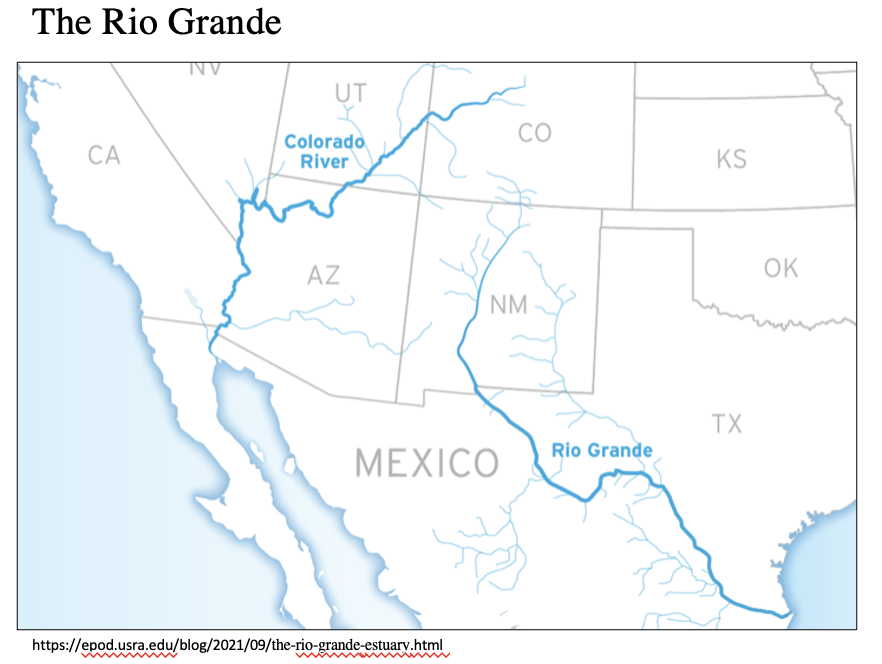
\includegraphics[width=0.75\linewidth]{image1_riogrande} \end{center}

\begin{center}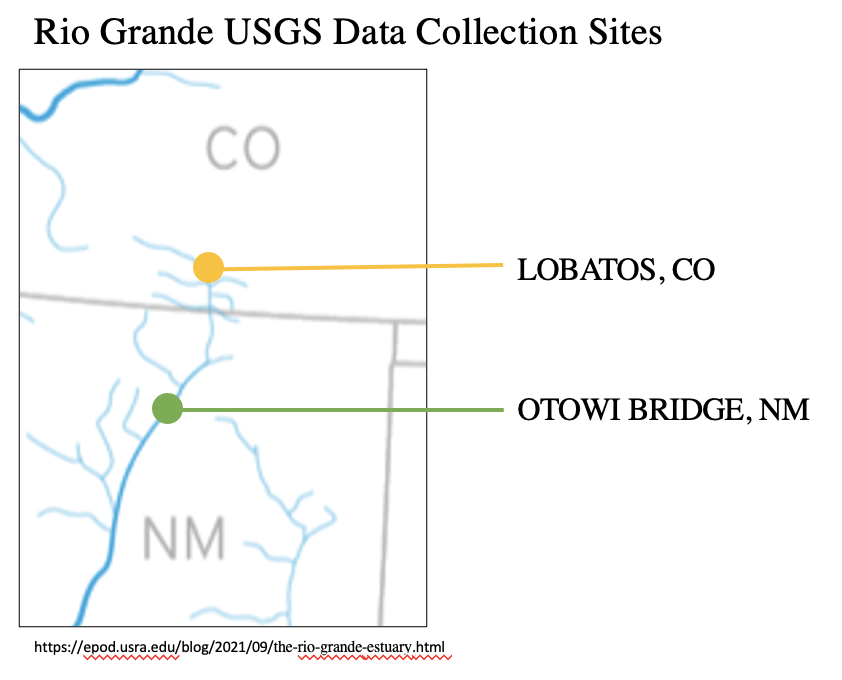
\includegraphics[width=0.75\linewidth]{image2_datacollectionsites} \end{center}
\newpage

\hypertarget{dataset-information}{%
\section{Dataset Information}\label{dataset-information}}

The data for this analysis was taken for USGS stream gauge data base
between 2000-2021 at two different locations, Lobatos, CO and Otowi
Bridge, NM, USGS code numbers 08251500 and 08313000 respectively. At
Lobatos, CO data was collected for total phosphorus in the water in
mg/L. At Otowi Bridge, NM data was collected for suspended sedimentation
concentration in the water also in mg/L. Additionally, discharge data in
cfs was collected for both sites. It was difficult to locate gauge
stations on the upper Rio Grande that had both phosphorus and
sedimentation data for the the desired period of time. Consistent data
from the same gauge station for this period was unavailable, thus two
different gauge locations where used. Sedimentation data at Otowi Bridge
is daily data for the entire time period. Phosphorus data at Lobatos was
only available for roughly 6 months out of the year, every year. This
was the most consistent phosphorus sampling data found. Discharge data
was available for for the entire time period.

\begin{table}
\centering
\begin{tabular}[t]{l|l|r|r|l}
\hline
\multicolumn{5}{c}{Summary of Data} \\
\cline{1-5}
Site & Parameter & Observations & Code & Units\\
\hline
Lobatos, CO & Phosphorus & 229 & 8251500 & mg/L\\
\hline
Lobatos, CO & Discharge & 229 & 8251500 & cfs\\
\hline
Otowi, NM & Sedimentation & 3509 & 8313000 & mg/L\\
\hline
Otowi, NM & Discharge & 3509 & 8313000 & cfs\\
\hline
\end{tabular}
\end{table}

The data was read in directly from the USGS data base using functions
whatNWISdata and readWQPqw. Wrangling the water quality data required
reading in all available water quality parameters and filtering the
dataset for the desired parameters. Data was grouped and summarised by
day, columns were renamed and NA's were dropped from the data set. The
data frame was pivoted from longer to wider and joined with the selected
parameters from the discharge dataset for each location. Further into
the analysis, the location data ets were split into pre and post water
fund implementation, 2001-2007 and 2008-2021 respectively.

\newpage

\hypertarget{exploratory-analysis}{%
\section{Exploratory Analysis}\label{exploratory-analysis}}

The data for each site was explored over the entire time period captured
and for the pre and post water fund periods for each water parameter. A
visual analysis of line graphs of the data appear to reveal some
characteristics of the how the Rio Grande water quantity and quality is
changing.

\hypertarget{lobatos-co}{%
\subsection{Lobatos, CO}\label{lobatos-co}}

At the Lobatos gauge site there seems to be a trend of decreasing
discharge over time as well as well as a slight decreasing trend in
phosphorus over time as well. A closer look at the pre and post fund
data shows this relationship at a finer scale. The project objectives
were to cause an increase in river discharge and a decrease in
phosphorus over time. This data shows that the project interventions did
not have an apparent effect on these water quantity and quality measures
a Lobatos.

\hypertarget{section}{%
\subsubsection{2007-2021}\label{section}}

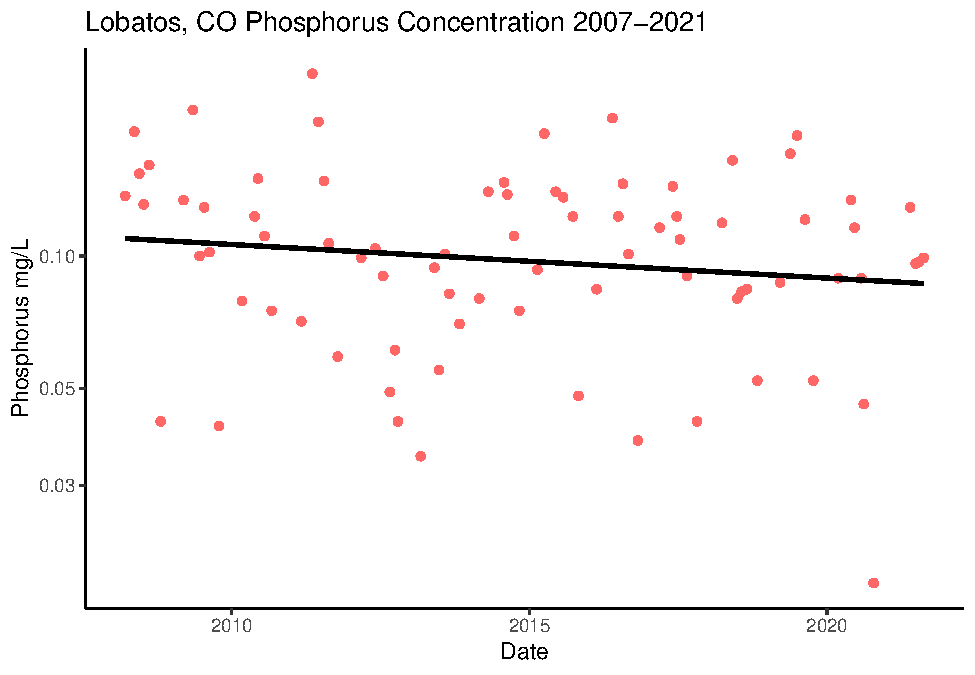
\includegraphics[width=0.5\linewidth]{Project_Template_files/figure-latex/2007-2021 looking at stream gauge data over time-1}
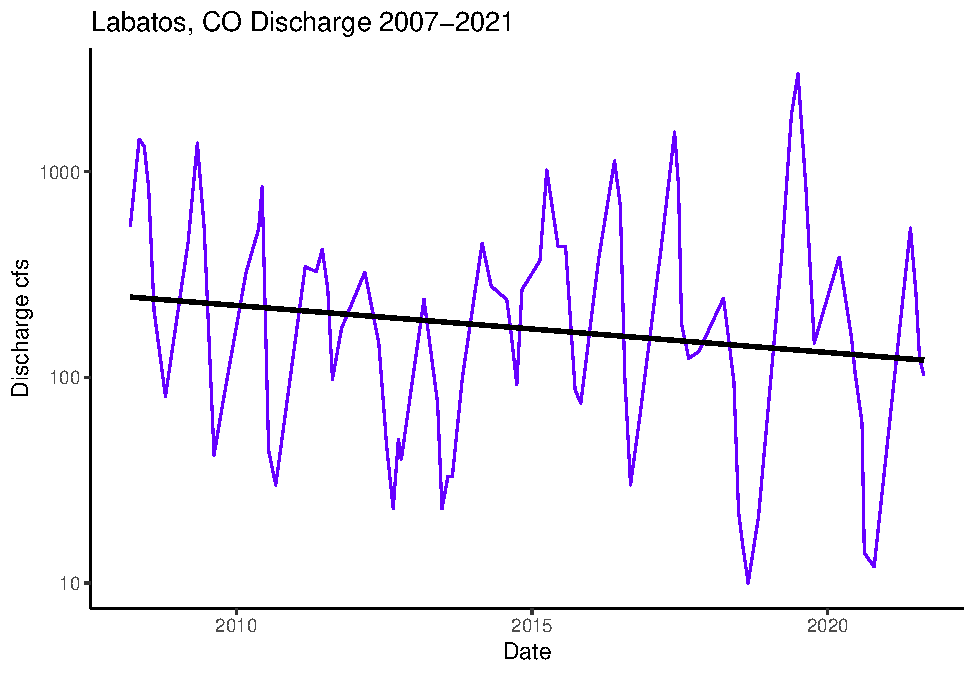
\includegraphics[width=0.5\linewidth]{Project_Template_files/figure-latex/2007-2021 looking at stream gauge data over time-2}
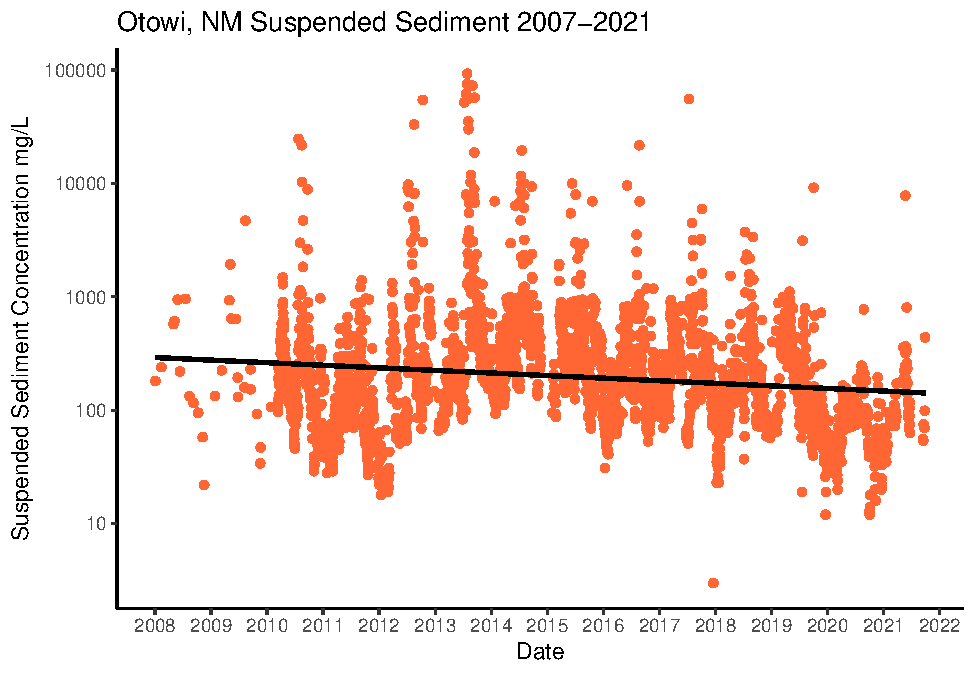
\includegraphics[width=0.5\linewidth]{Project_Template_files/figure-latex/2007-2021 looking at stream gauge data over time-3}
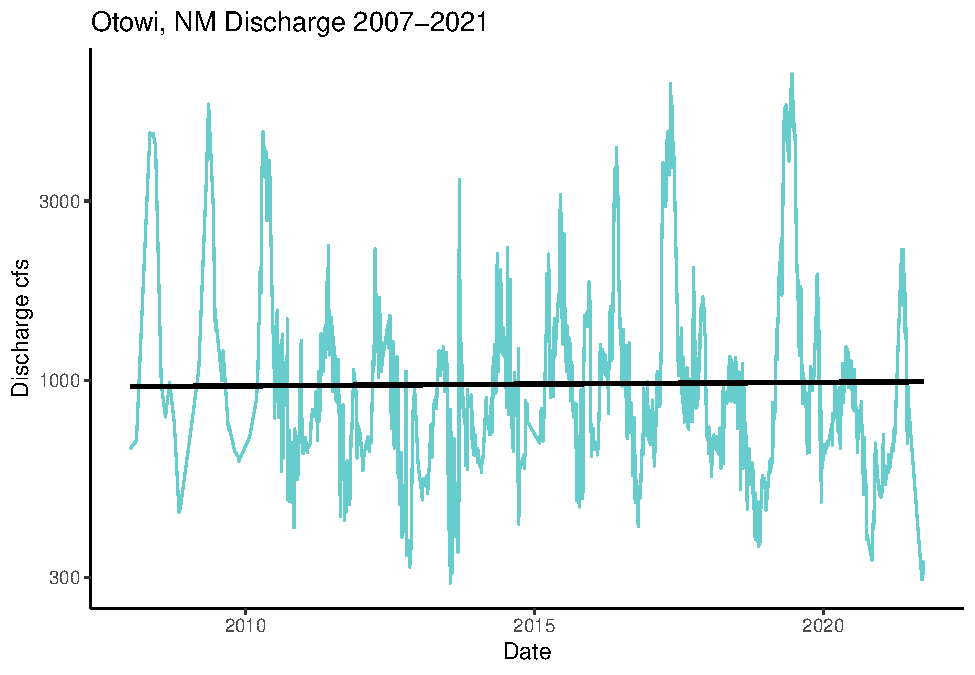
\includegraphics[width=0.5\linewidth]{Project_Template_files/figure-latex/2007-2021 looking at stream gauge data over time-4}

\hypertarget{section-1}{%
\subsubsection{2007-2014}\label{section-1}}

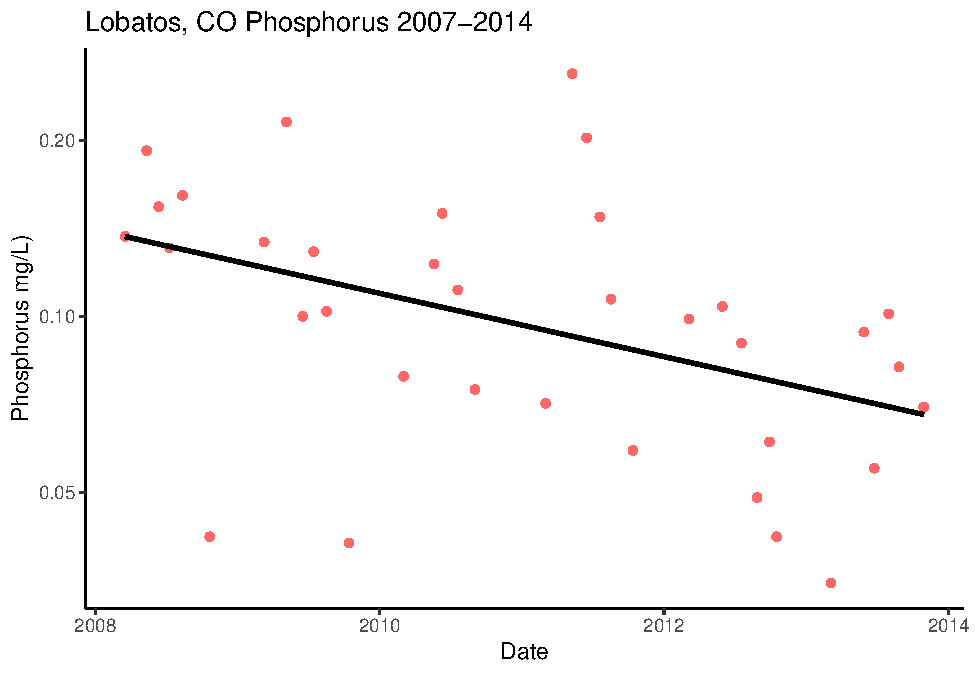
\includegraphics[width=0.5\linewidth]{Project_Template_files/figure-latex/2007-2014 looking at stream gauge data over time-1}
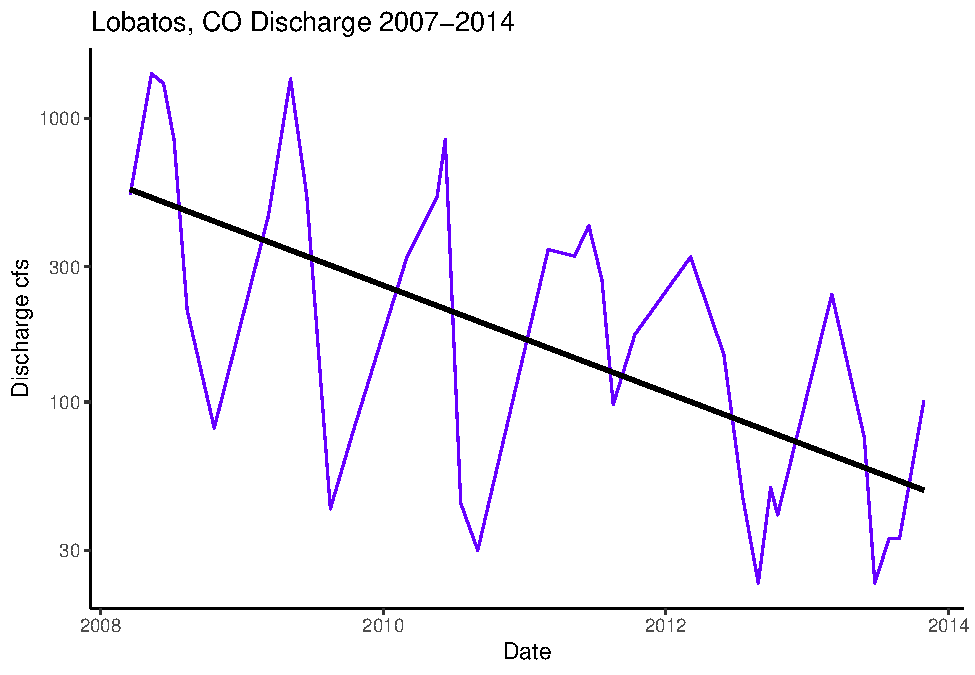
\includegraphics[width=0.5\linewidth]{Project_Template_files/figure-latex/2007-2014 looking at stream gauge data over time-2}
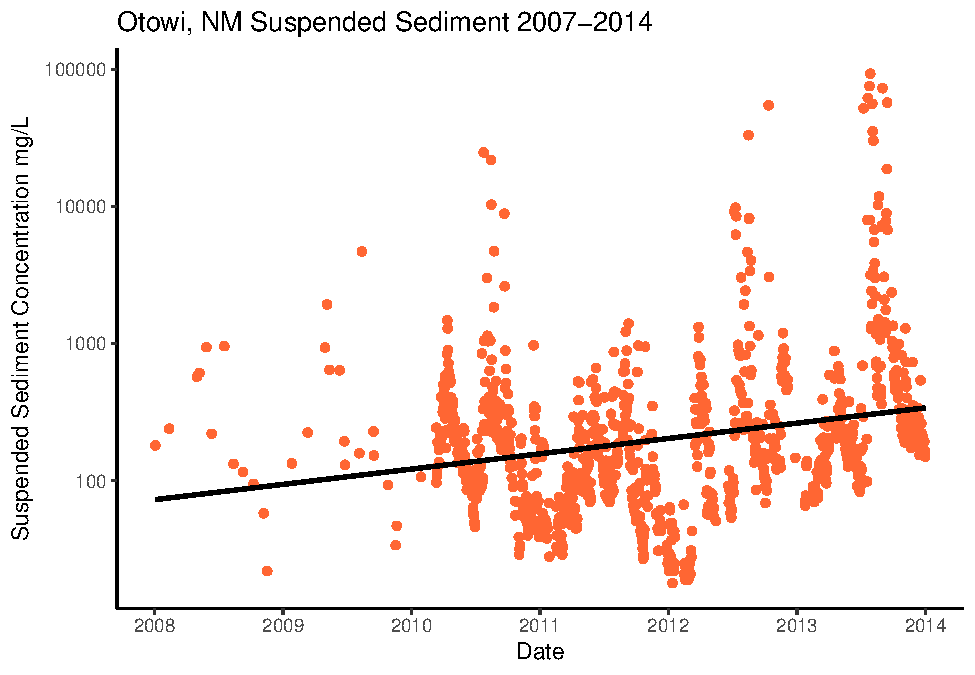
\includegraphics[width=0.5\linewidth]{Project_Template_files/figure-latex/2007-2014 looking at stream gauge data over time-3}
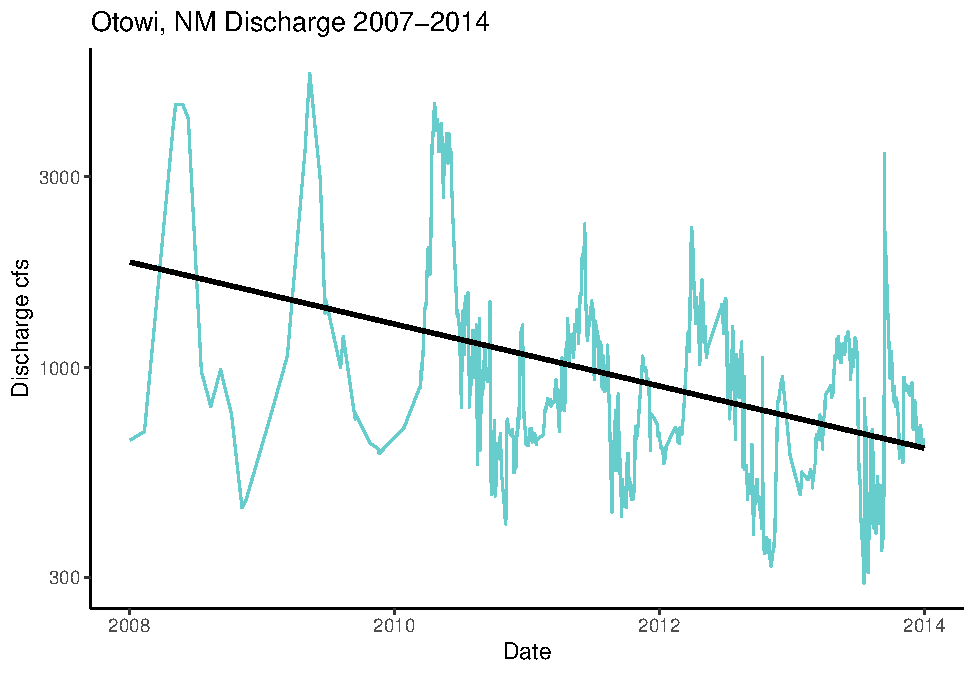
\includegraphics[width=0.5\linewidth]{Project_Template_files/figure-latex/2007-2014 looking at stream gauge data over time-4}

\hypertarget{section-2}{%
\subsubsection{2014-2021}\label{section-2}}

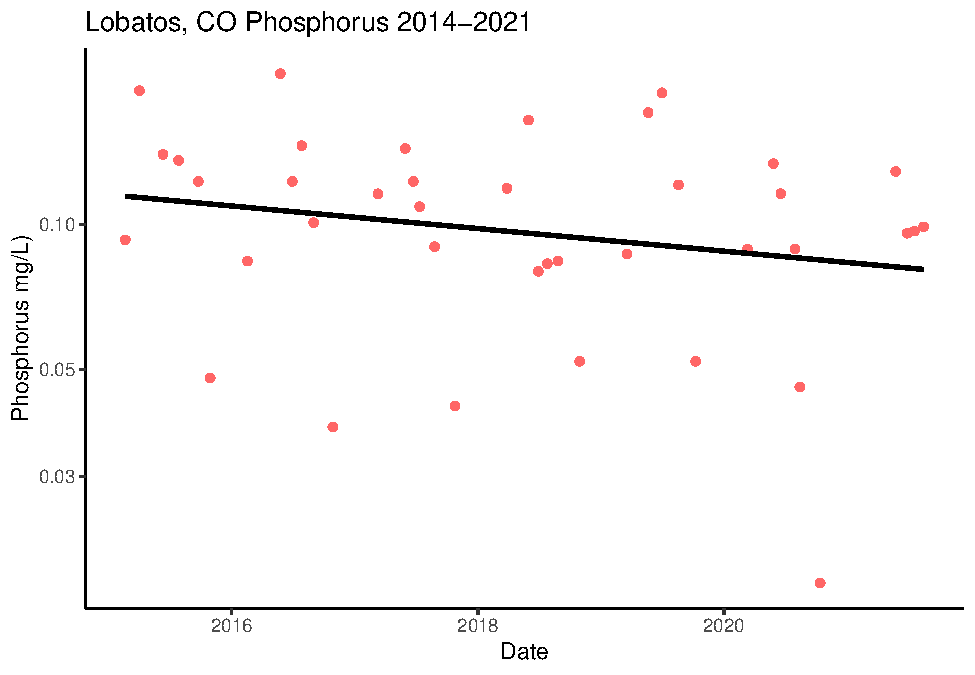
\includegraphics[width=0.5\linewidth]{Project_Template_files/figure-latex/2014-2021 looking at stream gauge data over time-1}
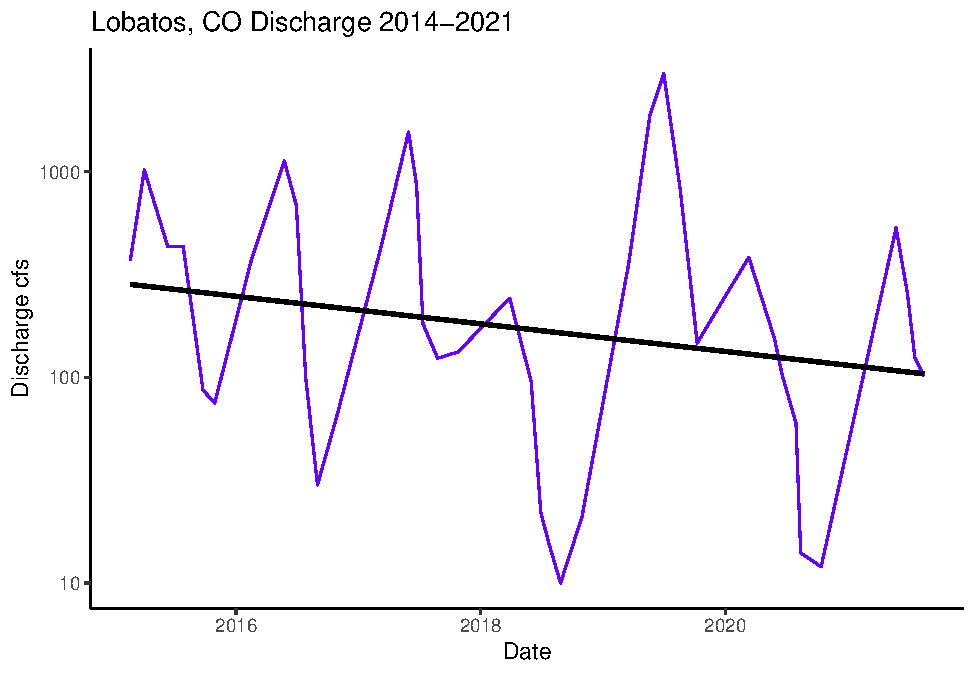
\includegraphics[width=0.5\linewidth]{Project_Template_files/figure-latex/2014-2021 looking at stream gauge data over time-2}
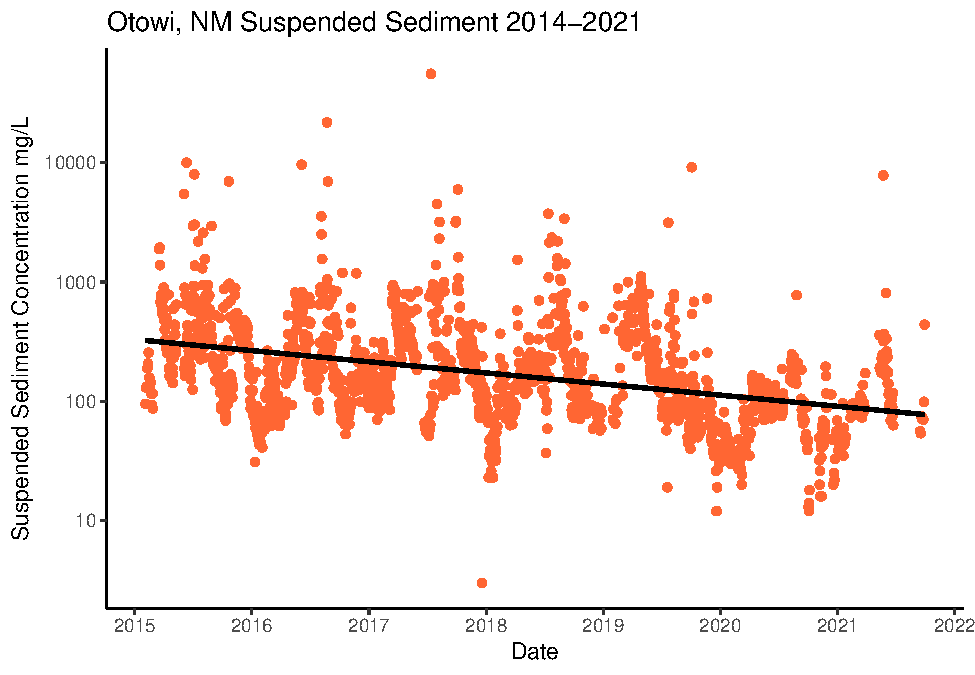
\includegraphics[width=0.5\linewidth]{Project_Template_files/figure-latex/2014-2021 looking at stream gauge data over time-3}
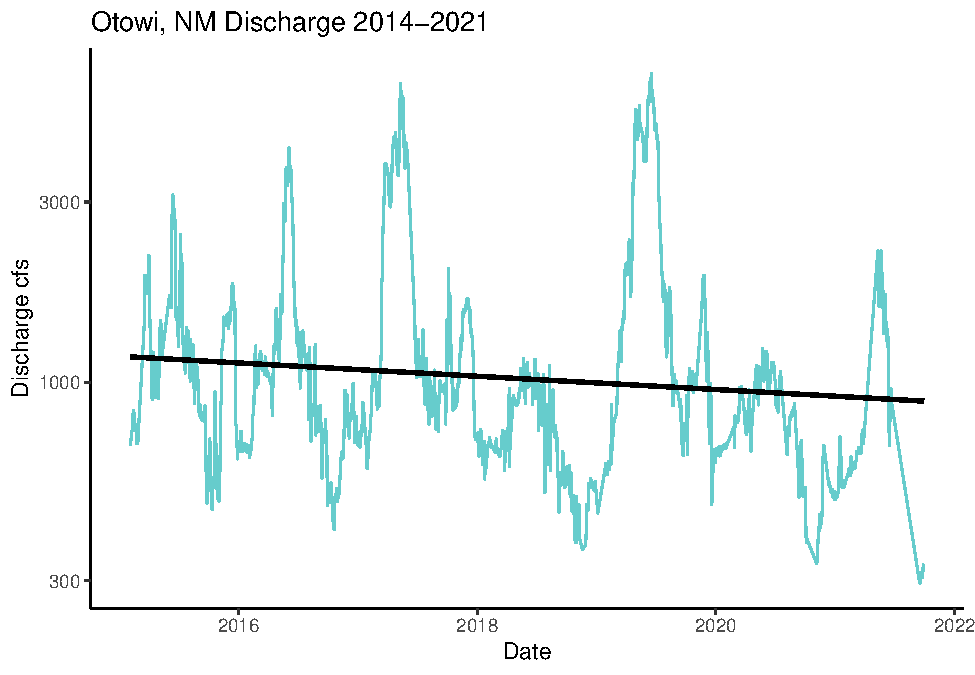
\includegraphics[width=0.5\linewidth]{Project_Template_files/figure-latex/2014-2021 looking at stream gauge data over time-4}

\hypertarget{otowi-bridge-nm}{%
\subsection{Otowi Bridge, NM}\label{otowi-bridge-nm}}

At the Otowi Bridge gauge site there does not seem to be a trend in
discharge data over the entire time period, but in both the pre and post
fund scenarios a negative discharge trend appears. The Project was
hoping to see an increase in river discharge after project was
implemented. These results are not showing that the project
interventions were successful in this way. The sedimentation data
appears to show an increasing trend in sediment load before the fund
implementation and a decreasing trend in sedimentation after the fund
was implemented, right around 2014/2015. This infers that the
restoration projects are succeeding in reducing sediment load and
improving water quality in this regard.

\newpage

\hypertarget{analysis}{%
\section{Analysis}\label{analysis}}

Further analysis of the data involved investigating if there is a linear
relationship between phosphorus levels in the water and discharge, as
well as sedimentation levels in the water and discharge. The results of
both linear models resulted in significant positive relationships
between these variables (p\textless{} 0.05). As discharge increases
there are higher levels of phosphorus and sedimentation in the water.

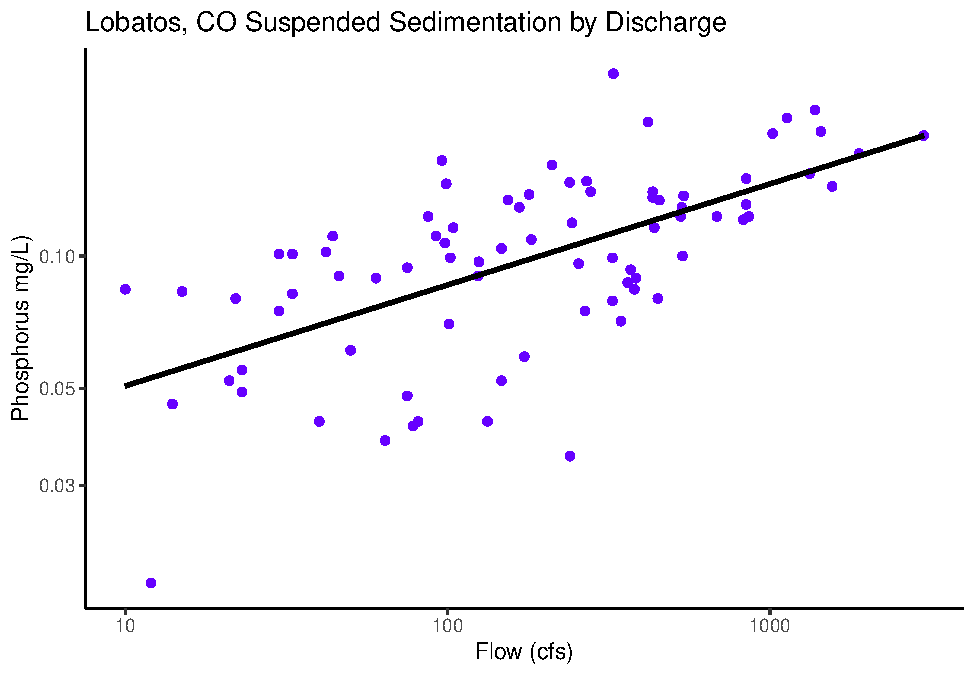
\includegraphics{Project_Template_files/figure-latex/unnamed-chunk-4-1.pdf}

Additional analysis was also preformed to explore trends over time at
Otowi Bridge. The initial exploratory analysis indicated there would be
a decreasing trend in sedimentation beginning around the fund
implementation time. To see if this relationship is significant a
Seasonal Man Kendall (SMK) test was preformed. A SMK test is appropriate
for this location given there is monthly data available for all years
and there is a seasonal trend in the data. The SMK test revealed that
there is not a significant relationship in sedimentation or discharge
over time before the water fund was implemented (p\textgreater{} 0.05),
nor for discharge over time after fund implementation (p\textgreater{}
0.05). However, the SMK test resulted is a nearly significant
relationship in sedimentation over time after 2014 (p=.07). This further
analysis indicates that although the inital analysis seems to reveal
positive relationships in the data, the trends are not significant.

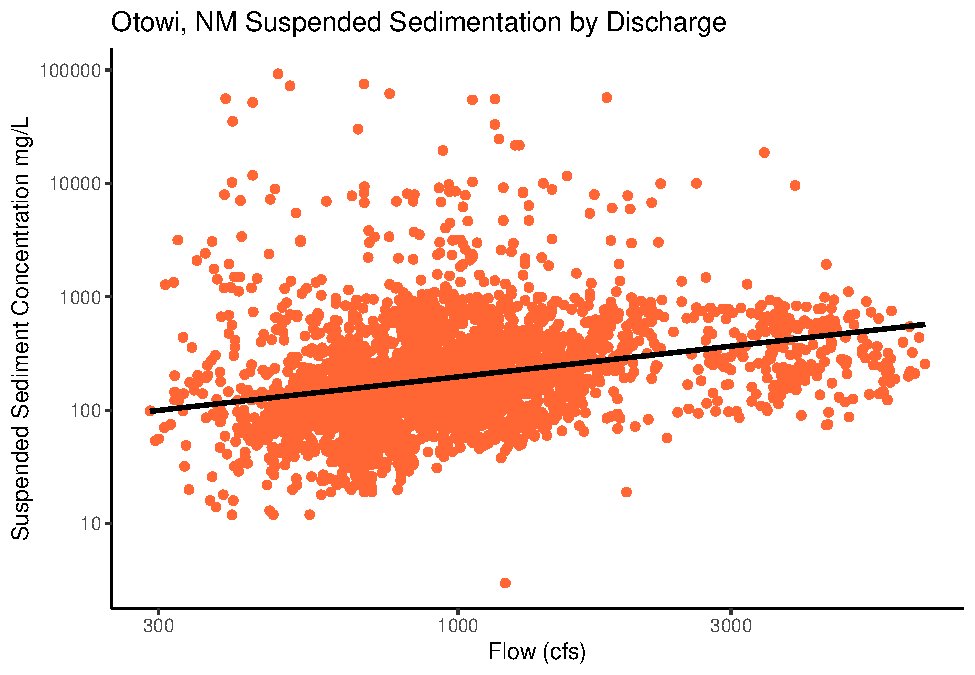
\includegraphics{Project_Template_files/figure-latex/unnamed-chunk-6-1.pdf}

Research questions 1 and 2 were answered through this analysis. 1. Water
quantity has not increased in the river since the fund was implemented.
2. Water quality has increased in the river since the fund was
implemented, but not significantly. Specifically, suspended sediment as
decreased slightly, and phosphorus has continued an a very slight
decreasing trend since prior to fund implementation.

\newpage

\hypertarget{summary-and-conclusions}{%
\section{Summary and Conclusions}\label{summary-and-conclusions}}

Although the restoration interventions implemented through the water
fund creation appeared to achieve their objectives, relationships were
not significant. Water funds are put in place to be active for decades
if not into perpetuity. Therefore, this water fund and it's operations
are young. The 600,000 acres of forest have not all be restored. There
is potential for increased impact to be observed after more time.

Water fund models are extensively researched before their implementation
and are specifically tailored to the project location. These models have
had great success achieving their desired outcomes in various watersheds
around the world. Further analysis should be completed at a later date
to confirm if the project interventions are successful.

\newpage

\hypertarget{references}{%
\section{References}\label{references}}

The Nature Conservancy. (2020). Rio grande water
fund.https://www.nature.org/en-us/about-us/where-we-work/united-states/new-mexico/stories-in-new-mexico/new-mexico-rio-grande-water-fund/

\end{document}
